%----------------------------------------------------------------------------------------
%	PACKAGES AND OTHER DOCUMENT CONFIGURATIONS
%----------------------------------------------------------------------------------------

\documentclass[
	a4paper, % Paper size, use either a4paper or letterpaper
	10pt, % Default font size, can also use 11pt or 12pt, although this is not recommended
	unnumberedsections, % Comment to enable section numbering
	twoside, % Two side traditional mode where headers and footers change between odd and even pages, comment this option to make them fixed
]{LTJournalArticle}

\addbibresource{sample.bib} % BibLaTeX bibliography file

\runninghead{} % A shortened article title to appear in the running head, leave this command empty for no running head

\footertext{} % Text to appear in the footer, leave this command empty for no footer text

\setcounter{page}{1} % The page number of the first page, set this to a higher number if the article is to be part of an issue or larger work

%----------------------------------------------------------------------------------------
%	TITLE SECTION
%----------------------------------------------------------------------------------------

\title{CSPB 3202 HW 5 - Kaggle Competition\\} % Article title, use manual lines breaks (\\) to beautify the layout

% Authors are listed in a comma-separated list with superscript numbers indicating affiliations
% \thanks{} is used for any text that should be placed in a footnote on the first page, such as the corresponding author's email, journal acceptance dates, a copyright/license notice, keywords, etc
\author{%
	Taylor Larrechea
}

% Affiliations are output in the \date{} command
\date{\footnotesize\ The University Of Colorado Boulder, College Of Engineering And Applied Science}

% Full-width abstract
\renewcommand{\maketitlehookd}{
	\begin{abstract}
		This assignment focuses on training a Machine Learning model that can accurately classify images that represent cancer. For this model, the python package \textit{Tensorflow} was used to train the model.
		This article will discuss the methodology used to train the model, the results of the model, and the conclusions that can be drawn from the results.
	\end{abstract}
}

%----------------------------------------------------------------------------------------

\begin{document}

\maketitle % Output the title section

%----------------------------------------------------------------------------------------
%	ARTICLE CONTENTS
%----------------------------------------------------------------------------------------

\section{Imports}

The first step that was used in creating a model to classify images was to import the necessary libraries. The libraries that were imported and used in this model were:

\begin{itemize}
	\item \textbf{pandas}
	\item \textbf{tensorflow}
	\begin{itemize}
		\item \textbf{keras.preprocessing.image} - ImageDataGenerator: A class that generates batches of tensor image data with real-time data augmentation.
		\item \textbf{keras.applications} - ResNet50: A pre-trained model that can be used to classify images.
		\item \textbf{keras.models} - Model: A class that groups layers into an object with training and inference features.
		\item \textbf{keras.layers}
		\begin{itemize}
			\item \textbf{GlobalAveragePooling2D}: A class that applies average pooling on the spatial dimensions until each spatial dimension is one.
			\item \textbf{Dense}: A class that implements the operation: output = activation(dot(input, kernel) + bias) where activation is the element-wise activation function passed as the activation 
			argument, kernel is a weights matrix created by the layer, and bias is a bias vector created by the layer (only applicable if use\_bias is True).
			\item \textbf{Input}: A class that is used to instantiate a Keras tensor.
		\end{itemize}
		\item \textbf{keras.callbacks}:
		\begin{itemize}
			\item \textbf{ModelCheckpoint}: A class that saves the model after every epoch.
		\end{itemize}
	\end{itemize}
\end{itemize}

Once these models were imported, the model was now set to be trained.

\section{Model Training}

To begin training this model, the first step was to get the data from the CSV file that was provided by Kaggle.

\subsection{Data Preprocessing}

The name of the CSV file that was provided was \textit{train\_labels.csv}. This file was loaded into a pandas DataFrame where label was loaded into one column and the image ID was loaded into another
column.

This data was then split into a training and validation set. The training set was 80\% of the data and the validation set was 20\% of the data. The intention of using a validation set was an attempt to
prevent overfitting of the model.

\subsection{Data Augmentation}

The next step was to then augment the data that was loaded. This was done using the \textit{ImageDataGenerator} class from the \textit{keras.preprocessing.image} module. This class was used to generate
batches of tensor image data with real-time data augmentation. The data augmentation that was used was to rescale the images by 1/255, rotate the images by 20 degrees, zoom the images by 20\%, and flip
the images horizontally.

\subsection{Model Creation}

After the data was processed and then subsequently augmented, the next step was to create the model. The model that was used was the ResNet50 model from the \textit{keras.applications} module. This model
was used because it is a pre-trained model that can be used to classify images. The model was then set to be trained on the training data. This model was then trained with a total of 10 epochs. The results
of each subsequent epoch were saved using the \textit{ModelCheckpoint} class from the \textit{keras.callbacks} module. This model was then saved using the \textit{model.save()} method. 

\section{Model Results}

After the model was created, the next step was to evaluate the model. This was achieved by loading the saved model that was previously created and evaluating it in a separate file. 

\subsection{Model Training}

The results from the 10 epochs that were trained can be seen in the table below:

\begin{table}[ht]
	\centering
	\begin{tabular}{|c|c|c|c|c|}
		\hline
		\textbf{\#} & \textbf{T. Acc} & \textbf{T. Loss} & \textbf{V. Acc} & \textbf{V. Loss} \\ \hline
		1 & 0.5981 & 0.6611 & 0.6655 & 0.6245 \\ \hline
		2 & 0.6555 & 0.6204 & 0.6942 & 0.6078 \\ \hline
		3 & 0.6774 & 0.6048 & 0.6947 & 0.5972 \\ \hline
		4 & 0.6928 & 0.5944 & 0.6949 & 0.5890 \\ \hline
		5 & 0.6948 & 0.5885 & 0.7049 & 0.5863 \\ \hline
		6 & 0.6977 & 0.5855 & 0.7025 & 0.5819 \\ \hline
		7 & 0.7032 & 0.5799 & 0.7099 & 0.5756 \\ \hline
		8 & 0.7038 & 0.5789 & 0.7086 & 0.5761 \\ \hline
		9 & 0.7062 & 0.5751 & 0.7096 & 0.5739 \\ \hline
		10 & 0.7087 & 0.5720 & 0.7058 & 0.5715 \\ \hline
	\end{tabular}
	\caption*{Training And Validation Results}
\end{table}

We can visualize the results of the epoch accuracy and loss below:

\begin{center}
	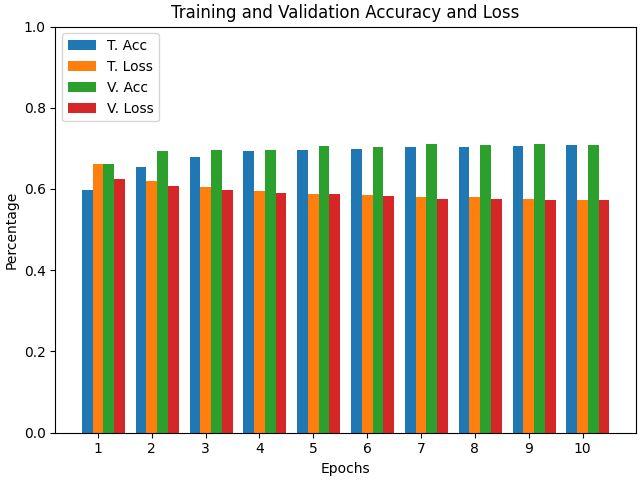
\includegraphics[width=0.45\textwidth]{Figures/Epoch Results Graph.png}
\end{center}

After all 10 epochs were trained, the final values for the accuracy and loss were:

\begin{itemize}
	\item \textbf{Training Accuracy:} 0.7087
	\item \textbf{Training Loss:} 0.5720
	\item \textbf{Validation Accuracy:} 0.7058
	\item \textbf{Validation Loss:} 0.5715
\end{itemize}

From the beginning to the end of the training, the model improved in accuracy and loss. The total change of the values were:

\begin{itemize}
	\item \textbf{Training Accuracy Change:} 0.1106
	\item \textbf{Training Loss Change:} 0.0891
	\item \textbf{Validation Accuracy Change:} 0.0403
	\item \textbf{Validation Loss Change:} 0.0530
\end{itemize}

\subsection{Model Evaluation}

After the model was trained with the 10 epochs, it was evaluated and the results were put into a CSV. Since there are 57,458 images in the test set, it is impractical to show the results in a table
format. Instead, the results of the \textit{label} column were plotted in a histogram.

\begin{center}
	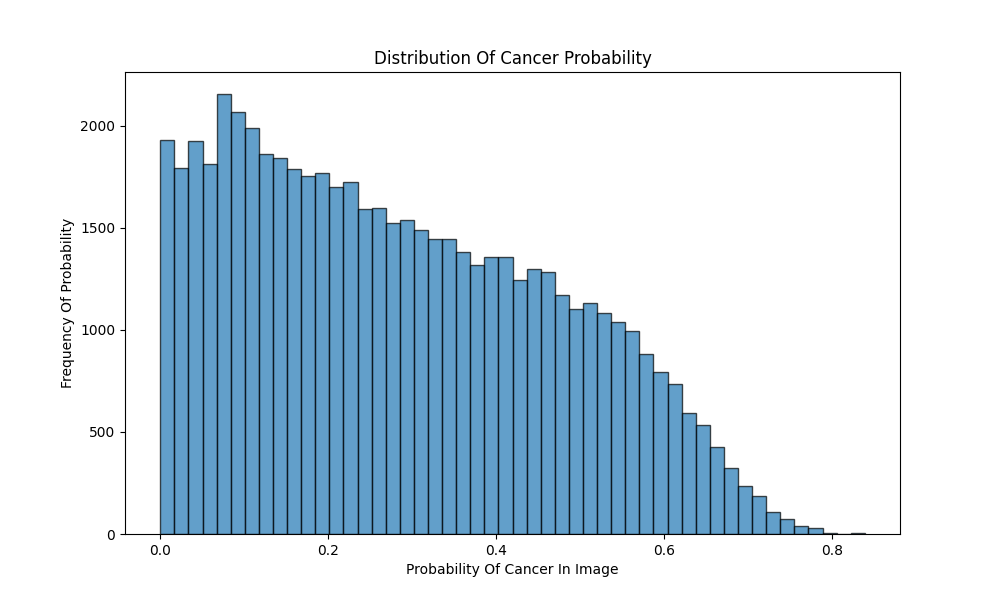
\includegraphics[width=0.5\textwidth]{Figures/Positive Cancer Probability.png}
\end{center}

The above image shows a frequency of probability distributions found from the model evaluation. On the x-axis, the probability of the image being positive for cancer is shown. On the y-axis, the frequency
of the given probability is shown.

\subsection{Kaggle Submission}

After the model was evaluated, the results were put into a CSV file and then submitted to Kaggle. The screenshot from the Kaggle submission can be seen below:

\begin{center}
	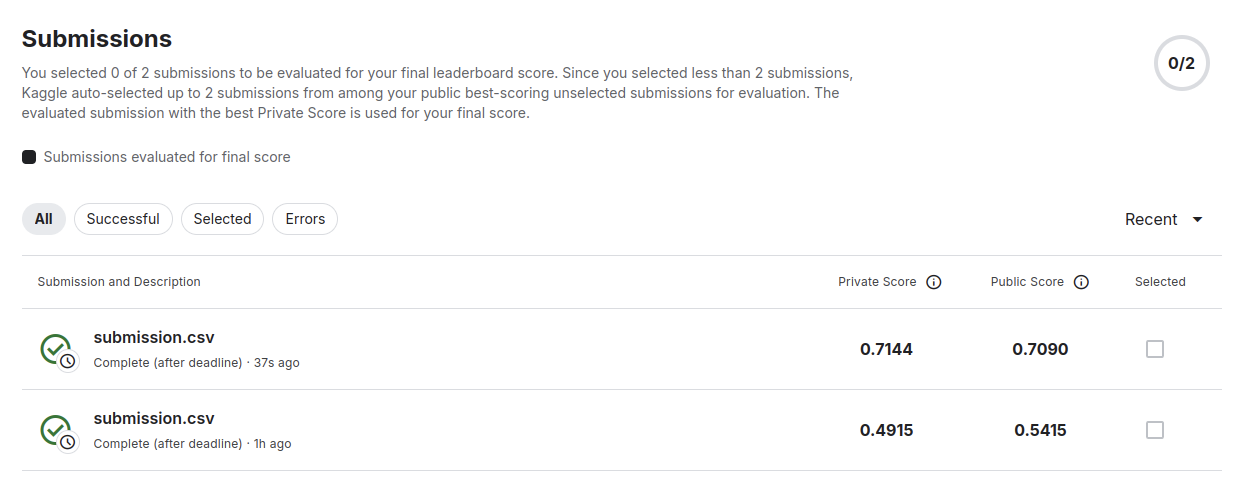
\includegraphics[width=0.5\textwidth]{Figures/Kaggle Results - Individual.png}
\end{center}

Due to the Kaggle competition being closed, the results from this model were not able to be placed on the leader board. The final public score of this competition was \textbf{0.7090}.

\section{Conclusion}

In conclusion, the model that was created was able to classify images that represented cancer with an accuracy of 70.90\%. This model was trained with 10 epochs and was able to improve in accuracy and loss
and generally performed pretty well. Considering that the model was trained with a pre-trained model, the results were pretty good. The model was able to classify images with a high degree of accuracy and
if more fine tuning were possible, the model could have performed even better.

\subsection{GitHub Repository}

The source code that was used to create this model can be found in the following GitHub repository:

\begin{itemize}
	\item \href{https://github.com/QuantumCompiler/Kaggle-Cancer-Competition}{QuantumCompiler - Kaggle Cancer Competition}
\end{itemize}

\end{document}